%%
% Modificación de una plantilla de Latex para adaptarla al castellano.
%%

%%%%%%%%%%%%%%%%%%%%%
% Thin Sectioned Essay
% LaTeX Template
% Version 1.0 (3/8/13)
%
% This template has been downloaded from:
% http://www.LaTeXTemplates.com
%
% Original Author:
% Nicolas Diaz (nsdiaz@uc.cl) with extensive modifications by:
% Vel (vel@latextemplates.com)
%
% License:
% CC BY-NC-SA 3.0 (http://creativecommons.org/licenses/by-nc-sa/3.0/)
%
%%%%%%%%%%%%%%%%%%%%%

%----------------------------------------------------------------------------------------
%	PACKAGES AND OTHER DOCUMENT CONFIGURATIONS
%----------------------------------------------------------------------------------------

\documentclass[a4paper, 10pt]{article} % Font size (can be 10pt, 11pt or 12pt) and paper size (remove a4paper for US letter paper)
\usepackage{helvet}
\renewcommand{\familydefault}{\sfdefault}
\usepackage[protrusion=true,expansion=true]{microtype} % Better typography
\usepackage{graphicx} % Required for including pictures
\usepackage[usenames,dvipsnames]{color} % Coloring code
\usepackage{wrapfig} % Allows in-line images
\usepackage[utf8]{inputenc}
\usepackage{enumerate}
\usepackage{enumitem}

% Imágenes
\usepackage{graphicx} 

\usepackage{amsmath}
% para importar svg
%\usepackage[generate=all]{svgfig}

% sudo apt-get install texlive-lang-spanish
\usepackage[spanish]{babel} % English language/hyphenation
\selectlanguage{spanish}
% Hay que pelearse con babel-spanish para el alineamiento del punto decimal
\decimalpoint
\usepackage{dcolumn}
\newcolumntype{d}[1]{D{.}{\esperiod}{#1}}
\makeatletter
\addto\shorthandsspanish{\let\esperiod\es@period@code}
\makeatother

\usepackage{longtable}
\usepackage{tabu}
\usepackage{supertabular}

\usepackage{multicol}
\newsavebox\ltmcbox

% Para algoritmos
\usepackage{algorithm}
\usepackage{algorithmic}
\usepackage{amsthm}

% Para matrices
\usepackage{amsmath}

% Símbolos matemáticos
\usepackage{amssymb}
\usepackage{accents}
\let\oldemptyset\emptyset
\let\emptyset\varnothing

\usepackage[hidelinks]{hyperref}

\usepackage[section]{placeins} % Para gráficas en su sección.
\usepackage[T1]{fontenc} % Required for accented characters
\usepackage{tikz}
\newenvironment{allintypewriter}{\ttfamily}{\par}
\setlength{\parindent}{0pt}
\parskip=8pt
\linespread{1.05} % Change line spacing here, Palatino benefits from a slight increase by default

\makeatletter
\renewcommand\@biblabel[1]{\textbf{#1.}} % Change the square brackets for each bibliography item from '[1]' to '1.'
\renewcommand{\@listI}{\itemsep=0pt} % Reduce the space between items in the itemize and enumerate environments and the bibliography
\newcommand{\imagen}[2]{\begin{center} \includegraphics[width=90mm]{#1} \\#2 \end{center}}
\newcommand{\RFC}[1]{\href{https://www.ietf.org/rfc/rfc#1.txt}{RFC-#1}}

\renewcommand{\maketitle}{ % Customize the title - do not edit title and author name here, see the TITLE block below
\begin{center} % Center align
{\Huge\@title} % Increase the font size of the title
\end{center}

\vspace{20pt} % Some vertical space between the title and author name

\begin{flushright} % Right align
{\large\@author} % Author name
\\\@date % Date

\vspace{40pt} % Some vertical space between the author block and abstract
\end{flushright}
\renewcommand{\baselinestretch}{0.5}

}
%----------------------------------------------------------------------------------------
%	TITLE
%----------------------------------------------------------------------------------------

\title{\textbf{Distribución de Poisson}\\ % Title
\vspace{20 pt}
} % Subtitle

\author{\textsc{Rafael Nogales Vaquero\\
Lothar Soto Palma} % Author
\\{\textit{Universidad de Granada}}} % Institution

\date{\today} % Date

%----------------------------------------------------------------------------------------
%\setcounter{secnumdepth}{3}
\usepackage{anysize}
\marginsize{3cm}{3cm}{2.5cm}{2.5cm}

\begin{document}
\maketitle
\tableofcontents
\setcounter{page}{1}
\pagebreak
\section{Deducción de función de densidad}
La distribución de Poisson expresa a partir de una frecuencia de ocurrencia media, la probabilidad de que ocurra un determinado número de eventos durante cierto periodo de tiempo. Se especializa en la probabilidad de ocurrencia de sucesos con probabilidades pequeñas. Es una distribución que sirve para modelar diferentes tipos de experimentos, como fenómenosen los que se espera que ocurra un suceso en específico como esperar el bus, o la llegada de clientes en deternimado servicio.

La distribución de Poisson es un caso particular del limite de la distribución binomial, podemos deducirlo de la siguiente representación geométrica:\\
\begin{center}
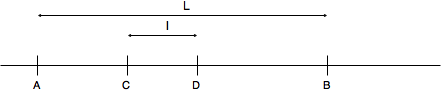
\includegraphics[scale=0.6]{1.png} 
\end{center}
Tomamos $AB$ como el segmento de longitud $L$ y $CD$ el segmento de longitud $l$ contenido en $AB$, la probabilidad de que un punto se encuentre en $CD$ es $l/L$. Sitomamos n puntos aleatorios en $AB$ la probabilidad de que exactamente $x$ de ellos esten en $CD$ viene dada por una distribución binomial:
$$B(x|\frac{l}{L},n)=\frac{n!}{x!(n-x)!}(\frac{l}{L})^x(1-\frac{l}{L})^{n-x}$$
n y L crecen indefinidamente de tal manera que el número promedio de puntos por unidad de longitud es un número finito $k \neq 0$, $\frac{n}{L}\rightarrow k$.
$$B(x|\frac{l}{L},n)=\frac{n(n-1)...(n-x+1)}{x!n^x}(\frac{nl}{L})^x(1-\frac{n}{L}\frac{l}{n})^{n-x}$$
asi que el limite de $B(x|\frac{l}{L},n)$ cuando $n,L\rightarrow \infty$:
$$\lim_{n,L\rightarrow \infty}B(x|\frac{l}{L},n) = \lim_{n,L\rightarrow \infty}\frac{1(1-\frac{1}{n})...(1-x+1\frac{x+1}{n})}{x!}(\frac{nl}{L})^x(1-\frac{n}{L}\frac{l}{n})^{n-x}=\frac{(kl)^xe^{-kl}}{x!}$$
Tomando que $kl=\theta$ obtenemos la expresión de la distribución de Poisson:
$$Poisson(\theta)=f(x|\theta)=\dfrac{e^{-\theta}\theta^x}{x!},\ \ \ x=0,1...$$
Tiene un único parámetro $\theta$ se suele denominar parámetro de intensidad, y se aplica sobre una variable aleatoria $X$.
\section{Función generatriz de momentos}
Para definir la función generatriz de momentos es importante ver que se verifica que $e^x=\sum_{i=0}^{\infty}\frac{x^i}{i!}$ es la serie de Taylor para $e^x$.
La función generatriz de momentos se define como sigue:
$$\phi(t)=E[e^{-tX}]=\sum_{x=0}^{\infty}e^{-t x}\frac{e^{-\theta}\theta^x}{x!}=e^{-\theta}\sum_{x=0}^{\infty}e^{t x}\frac{\theta^x}{x!}=e^{-\theta}\sum_{x=0}^{\infty}\frac{(\theta e^t)^x}{x!}=e^{-\theta}e^{\theta e^t}=e^{\theta(e^t-1)}$$
\subsection{Esperanza}
Para el calculo de la esperanza tan solo debemos derivar la función generatriz de momentos una vez y evaluarla con t=0:
$$\frac{\partial\phi}{\partial t} = \theta e^t e^{\theta(e^t-1)}$$
Evaluamos la expresión en t=0 y tenemos que:
$$E[X]=\theta$$
\subsection{Varianza}
La varianza tiene se puede expresar como $\sigma^2=E[X^2]-E[X]^2$ por lo que es tan solo calcular, usando la función generatriz de momentos, el momento de orden 2 por lo que volvemos a derivar la expresión anterior:
$$\frac{\partial^2\phi}{\partial t^2} = \theta e^t e^{\theta(e^t-1)}+\theta^2 e^{2t} e^{\theta(e^t-1)}$$
Evaluamos la expresión en t=0 y tenemos que:
$$E[X^2]=\theta+\theta^2$$
Y por lo tanto la expresión de la varianza es la siguiente:
$$\sigma^2=\theta+\theta^2-\theta^2=\theta$$

\subsection{Familia exponencial}
\section{EMV}

\subsection{Consistencia}
\subsection{Eficiencia}
\subsection{Insesgadez}
\subsection{Robustez}
\subsection{Suficiencia}
\subsection{Invarianza}
\section{Ejemplos}
\section{Referencias}
\end{document}